\documentclass[a4paper]{article}

\usepackage[utf8]{inputenc}
\usepackage[T1]{fontenc}
\usepackage{textcomp}
\usepackage{multicol}
\usepackage{verbatim,listings,minted}
\usepackage{mathtools,amssymb,amsthm}
\usepackage[a4paper, total={6in, 8in}]{geometry}
\usepackage[francais]{babel}

%============header and foot============
\usepackage{fancyhdr}
\pagestyle{fancy}
\renewcommand\headrulewidth{1pt}
\fancyhead[L]{\bfseries TP5 MDE}
% \fancyhead[R]{\includegraphics[scale=0.05]{image.png}}
\fancyfoot[L]{CHASSAGNOL Rémi}
\fancyfoot[R]{2023-2024}

%================image=================
\usepackage{graphicx}

%------------------------------------------------------------------------------%
%                                   document                                   %
%------------------------------------------------------------------------------%

\begin{document}
\begin{titlepage}
\begin{center}

    \textsc{\LARGE TP IDM}\\[0.5cm]

    {\huge \bfseries Génération de flux parallèles de nombres pseudo-aléatoires\\[3cm]}

      \centering
      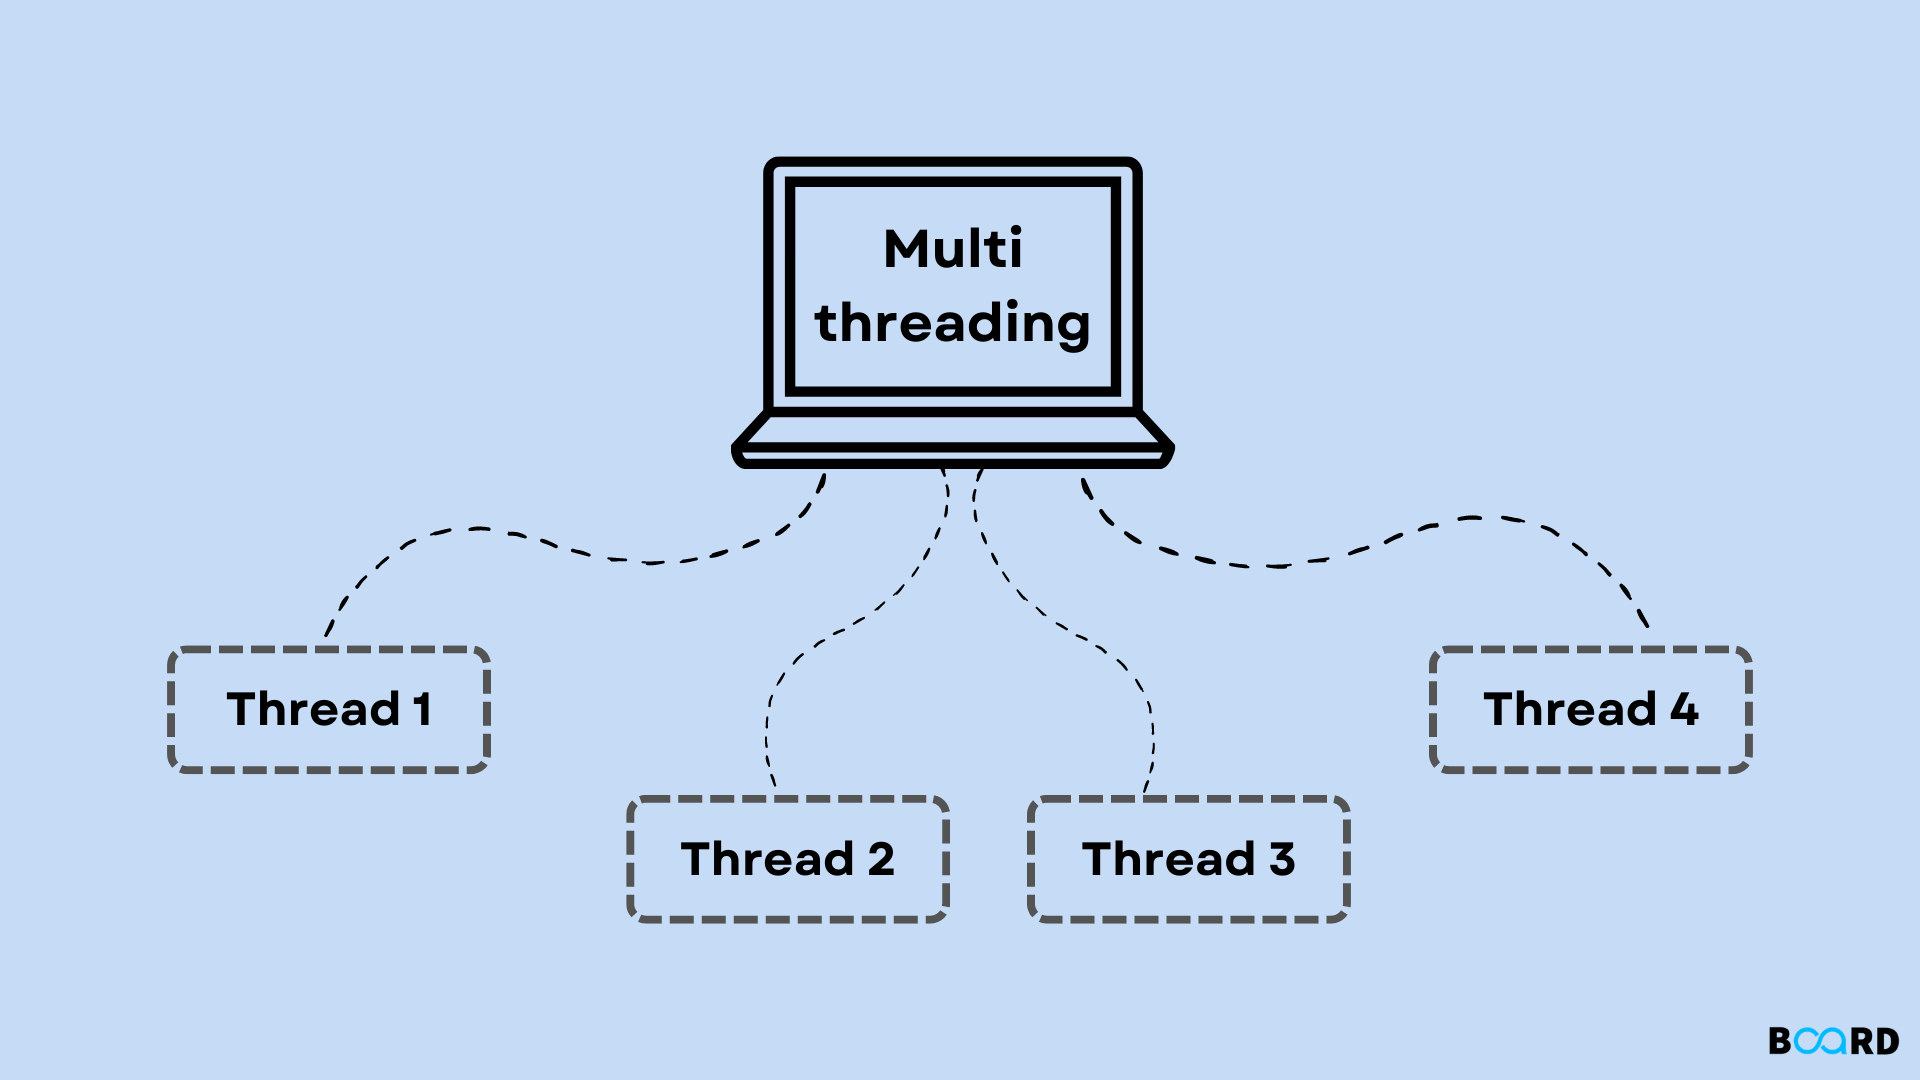
\includegraphics[scale=0.3]{./img/banner.png}

      \vspace*{\fill}

    \begin{multicols}{2}
      \large
      CHASSAGNOL Rémi\\

      \columnbreak

      \large
      \emph{Professeur:} HILL David\\
    \end{multicols}

    \textsc{\today}

  \end{center}
\end{titlepage}

\clearpage
\tableofcontents
\clearpage

\section{Introduction}

L'objectif de ce TP est d'utiliser le un générateur de nombres pseudo-aléatoires
pour réaliser des calculs en parallèle. Pour générer les nombres nous
utiliserons l'implémentation de Mersenne Twister fournie par la bibliothèque
CLHEP. Nous commencerons par détailler l'installation de la bibliothèque, puis
nous testerons la répétabilité des séquences de nombres générés aléatoirement.
Ensuite, nous traiterons l'exemple simple du calcul du nombre $\pi$, d'abord en
séquentiel, puis en parallèle. Avant de conclure, nous traiterons un exemple
plus complexe sur la génération de mots et de bases nucléiques.

\clearpage

\section{Utilisation de CLHEP}

Dans cette première section nous allons voir comment installer la bibliothèque
CLHEP. Pour simplifier la gestion des dépendances, ce projet utilise des
sous-modules git.

Le clonage des sous-modules ne se fait pas automatiquement lors du clonage du
projet. Pour avoir accès aux sous-modules, il faut utiliser les commandes
suivantes:

\begin{listing}[ht!]
\begin{minted}{bash}
  git submodule init
  git submodule update
\end{minted}
\caption{Synchronisation des sous-modules git.}
\label{lable}
\end{listing}

L'utilisation des sous-modules évite surcharger les serveurs contenant les
dépôts en stockant plusieurs fois le même code. De plus, ils permettent de
facilement cloner les dépendances (cela est plus simple que de télécharger la
bibliothèque manuellement).\\

Pour compiler la bibliothèque, il faut utiliser le script \lstinline{build.sh}
du répertoire \lstinline{lib}. Ce script va permettre de compiler et d'installer
la bibliothèque (fichiers d'entêtes, bibliothèque statiques, \dots) dans le
répertoire \lstinline{lib/CLHEP-lib}. Ensuite, on peut compiler le projet en
utilisant CMake.

\section{Test du générateur}

Avant de commencer les calculs, assurons-nous que le générateur produit bien
toujours les même séquences de nombres lorsqu'il charge les fichiers de
statuts.\\

La générations des fichier de statuts se fait avec la méthode
\lstinline{saveStatus} et le chargement des fichiers se fait avec la méthode
\lstinline{restoreStatus}. Dans la fonction \lstinline{question2}, nous générons
dans un premier temps des fichiers de statuts, et chaque statuts est séparé par
un certain nombre de tirage de nombre pseudo-aléatoires. Les tirages sont
sauvegardés dans un tableau.

Dans un second temps, nous restaurons les statuts et nous vérifions que les
tirages sont les même que ceux sauvegardés précédemment. Ici, nous utilisons un
\lstinline{assert} pour tester l'égalité des nombres. Si les nouveaux nombres
générés ne sont pas égaux à ceux sauvegardés, le programme s'arrête avec un code
erreur. Si le programme se termine sans échouer, le test du générateur est
valide.\\

À noter que ce test basique ne permet pas de valider avec certitude le bon
fonctionnement du générateur. Nous nous contenterons cependant de ce test étant
donné le fait la répétabilité de Mercenne Twister peut être prouvée
mathématiquement. Ici, nous vérifions juste que l'implémentation fonctionne sur
un petit nombre de tirages.

\section{Calcul de pi}

Maintenant que nous avons vérifier le bon fonctionnement du générateur, nous
allons réaliser un simple calcul de $\pi$ en utilisant la méthode de Monte
Carlo. Le calcul sera fait de façon séquentielle dans un premier temps, puis de
façon parallèle dans un second temps.

\subsection{Génération des fichiers de statuts}

Pour pouvoir paralléliser les calculs, il faut préalablement générer des
fichiers de statuts pour pouvoir lancer le générateur à partir d'un point donné.
Sans cette étape, les calculs lancés en parallèles utiliseront la même séquence
de nombre pseudo-aléatoires, ce qui rendra la parallélisation inutile.

\subsection{Calcul séquentiel}

\subsection{Calcul parallèle}

\subsubsection{Utilisation d'un script}

\subsubsection{Utilisation des threads}

\section{Gattaca}

\section{Conclusion}

\end{document}
